% Standalone source for figures/pipeline.pdf
\documentclass[tikz,border=3pt]{standalone}
\usepackage[T1]{fontenc}\usepackage{lmodern}
\usetikzlibrary{positioning,arrows.meta}
\begin{document}
\hyphenpenalty=10000
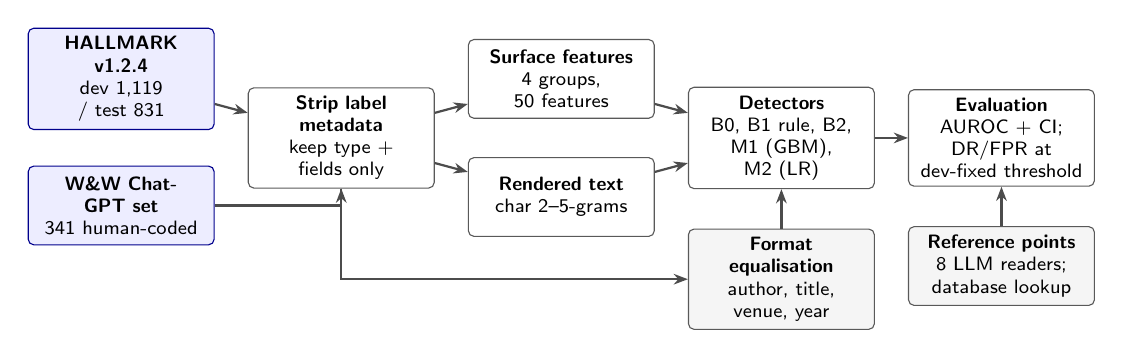
\begin{tikzpicture}[font=\sffamily\scriptsize,
  b/.style={draw=black!65, rounded corners=2pt, align=center, text width=2.15cm, minimum height=1.0cm, fill=white, inner sep=3pt},
  d/.style={b, fill=blue!7, draw=blue!55!black},
  r/.style={b, fill=black!4},
  a/.style={-{Stealth[length=1.8mm]}, thick, black!70}, node distance=0.45cm and 0.42cm]
\node[d] (h) {\textbf{HALLMARK v1.2.4}\\dev 1,119 / test 831};
\node[d, below=of h] (w) {\textbf{W\&W ChatGPT set}\\341 human-coded};
\node[b, right=of h, yshift=-0.75cm] (s) {\textbf{Strip label metadata}\\keep type + fields only};
\node[b, right=of s, yshift=0.75cm] (f) {\textbf{Surface features}\\4 groups, 50 features};
\node[b, right=of s, yshift=-0.75cm] (t) {\textbf{Rendered text}\\char 2--5-grams};
\node[b, right=of f, yshift=-0.75cm] (m) {\textbf{Detectors}\\B0, B1 rule, B2, M1 (GBM), M2 (LR)};
\node[b, right=of m] (e) {\textbf{Evaluation}\\AUROC + CI; DR/FPR at dev-fixed threshold};
\node[r, below=0.5cm of e] (x) {\textbf{Reference points}\\8 LLM readers; database lookup};
\node[r, below=0.5cm of m] (q) {\textbf{Format equalisation}\\author, title, venue, year};
\draw[a] (h) -- (s); \draw[a] (w) -| (s);
\draw[a] (s) -- (f); \draw[a] (s) -- (t); \draw[a] (f) -- (m); \draw[a] (t) -- (m); \draw[a] (m) -- (e);
\draw[a] (x) -- (e); \draw[a] (s.south) |- (q); \draw[a] (q) -- (m);
\end{tikzpicture}
\end{document}
